% !TeX program = pdfLaTeX
\documentclass[12pt]{article}
\usepackage{amsmath}
\usepackage{graphicx,psfrag,epsf}
\usepackage{enumerate}
\usepackage{natbib}
\usepackage{textcomp}
\usepackage[hyphens]{url} % not crucial - just used below for the URL
\usepackage{hyperref}
\providecommand{\tightlist}{%
  \setlength{\itemsep}{0pt}\setlength{\parskip}{0pt}}

%\pdfminorversion=4
% NOTE: To produce blinded version, replace "0" with "1" below.
\newcommand{\blind}{0}

% DON'T change margins - should be 1 inch all around.
\addtolength{\oddsidemargin}{-.5in}%
\addtolength{\evensidemargin}{-.5in}%
\addtolength{\textwidth}{1in}%
\addtolength{\textheight}{1.3in}%
\addtolength{\topmargin}{-.8in}%

%% load any required packages here



% Pandoc citation processing

\usepackage{booktabs}
\usepackage{longtable}
\usepackage{array}
\usepackage{multirow}
\usepackage{wrapfig}
\usepackage{float}
\usepackage{colortbl}
\usepackage{pdflscape}
\usepackage{tabu}
\usepackage{threeparttable}
\usepackage{threeparttablex}
\usepackage[normalem]{ulem}
\usepackage{makecell}
\usepackage{xcolor}

\begin{document}


\def\spacingset#1{\renewcommand{\baselinestretch}%
{#1}\small\normalsize} \spacingset{1}


%%%%%%%%%%%%%%%%%%%%%%%%%%%%%%%%%%%%%%%%%%%%%%%%%%%%%%%%%%%%%%%%%%%%%%%%%%%%%%

\if0\blind
{
  \title{\bf Trails Near Amherst College}

  \author{
        Nicole Frontero \\
    Department of Mathematics and Statistics, Amherst College\\
      }
  \maketitle
} \fi

\if1\blind
{
  \bigskip
  \bigskip
  \bigskip
  \begin{center}
    {\LARGE\bf Trails Near Amherst College}
  \end{center}
  \medskip
} \fi

\bigskip
\begin{abstract}
Given the ubiquity of geospatial data in modern life, independent study
into the basics of geospatial data is certainly warranted. In this
report, I provide background motivation for why the study of geospatial
data is so important. I then showcase a Shiny application that I created
that features a Leaflet map of the trails surrounding Amherst College.
In addition to describing the app functionality, I note the numerous
geospatial concepts that were essential to understand in order to make
the app. Finally, I conclude with reflections and future directions.
\end{abstract}

\noindent%
{\it Keywords:} geospatial data, Shiny, Leaflet
\vfill

\newpage
\spacingset{1.45} % DON'T change the spacing!

\hypertarget{introduction}{%
\section{Introduction}\label{introduction}}

\hypertarget{motivation}{%
\subsection{Motivation}\label{motivation}}

As a statistics and data science student, I have been trained in how to
extract information from data and how to present data in a
comprehensible manner. I have been exposed to parametric and
nonparametric statistical methods, static and dynamic methods for data
visualization, and computer science concepts, and yet, in part because
the fields of statistics, mathematics, and computer science are so
broad, I have not worked with geospatial data to date.

I have long had an interest in maps and globes. When I was in elementary
school, I used to enjoy spinning the globe that we had at home. I would
close my eyes as the globe spun, and I would use my finger to slow down
the globe's movement, acting as the brakes on the globe's movement. Once
the globe had stopped, I would try to guess the area of the world that
my finger had landed upon by noticing any raised surfaces denoting
mountainous regions. When I would open my eyes, I seldom had correctly
guessed the location (my predictive model was rather haphazard). Despite
my lack of accuracy, I would nevertheless relish in looking closer at
the given region of the globe, taking in the surrounding areas and
trying to commit it to memory. Given my longstanding interest in maps,
it feels fitting that I am dedicating my final project in
\href{https://www.amherst.edu/academiclife/departments/courses/2021F/STAT/STAT-495-2021F}{Statistics
495 - Advanced Data Analysis} to creating a map.

I have created a map of the trail systems surrounding Amherst College
that is accessible via a Shiny application that can be found
\href{https://nfrontero20.shinyapps.io/leaflet/}{here}. I wish that I
could have had access to a map like this during my time at Amherst
College, because then I would have learned about trails that I never
knew existed, and because I would have a sense of where the trails led
to instead of blindly following a trail.

This report serves as the final project in Statistics 495 - Advanced
Data Analysis, which is the final core curriculum course of the
Statistics major at Amherst College. Additionally, this project serves
as my having completed the comprehensive exam for the statistics major.
Most importantly, though, this project is a presentation of the
statistics and data science acumen that I have accrued throughout my
time as a statistics major at Amherst College.

\hypertarget{overview-of-the-report}{%
\subsection{Overview of the report}\label{overview-of-the-report}}

This report begins with background overview about geospatial data, in
which I define geospatial data and offer motivation into why it is
worthwhile to study geospatial data. I then showcase the Shiny app
through showing images of it, describing how the app was created the
geospatial concepts that I needed to understand in order to create it.
Finally, I conclude with some reflections and thoughts on future
directions.

\newpage

\hypertarget{background-information-on-working-with-geospatial-data}{%
\section{Background information on working with geospatial
data}\label{background-information-on-working-with-geospatial-data}}

\hypertarget{defining-geospatial-data}{%
\subsection{Defining geospatial data}\label{defining-geospatial-data}}

Geospatial data and geographic information system data are
closely-related types of data, but for the sake of clarity, I will
explicitly state the difference between them before I get too far into
this report. \emph{Geospatial data} refers to data that has some sort of
geographic component to it. This geographic component could come from
having data pertaining to coordinates, ZIP code, city, etc.
\citep{dempseyWhatDifferenceGIS2014a}. \emph{Geographic information
system} (hereafter referred to as GIS) data is a form of geospatial data
in which data is stored in layers. These layers can be manipulated,
analyzed, and visualized through mapping. Throughout this report, I'll
use the term geospatial data, but note that GIS data is the specific
type of geospatial data that I worked with.

\hypertarget{common-uses-of-geospatial-data}{%
\subsection{Common uses of geospatial
data}\label{common-uses-of-geospatial-data}}

Geospatial data is ubiquitous in modern life. To illustrate the
far-reaching influences of geospatial data on modern life, I'll share a
list of some of the ways in which I engage with geospatial data in a
given day, in hopes that it becomes apparent the multitude of ways in
which I rely upon geospatial data.

When I first wake up in the morning, I take a look outside my window to
see what the weather looks like. Regardless of what the weather is when
I wake up, I like to check a weather application on my phone so that I
can get a sense for what to expect the weather to be for the rest of the
day. A little later on my morning, I usually check the COVID-19 cases in
Massachusetts (where I live), the United States, and the entire world so
that I can stay up to date on the progression of the pandemic. When
trying to get information on COVID-19 cases, I tend to look at maps that
have color or bubble facets to help users gauge the scale of the
increase in cases in a given region.

Around midday when I'm having lunch, I often read the news or humor
myself with a funny video on YouTube, but I also may check Snapchat to
see if any of my friends have graced me with an image of their lives.
Sometimes when I am fumbling around with Snapchat and struggling to get
to the desired page within the app, I stumble across the
\href{https://map.snapchat.com/}{``Snap Map''} page, which shows where
my friends are located. I find this feature to be relatively invasive,
which is why I don't share my location, but that is neither here nor
there. In the afternoon, I might go for a run and when I do, I like to
use the \href{https://www.mapmyrun.com/us/}{MapMyRun} application on my
phone to track my run. Also, at some point during the day, I often end
up driving somewhere in the local area for some sort of errand, and
oftentimes, I'll use the mobile application for
\href{https://www.google.com/maps}{Google Maps} to help get me there.

Despite having bored you with a retelling of my day, note the many ways
in I engaged with geospatial data: for the weather, for navigation, for
estimation of travel time, for tracking the distance and pace of my run,
for staying up to date with COVID-19 cases, and even for tracking my
friends. The ways in which I tend to engage with geospatial data
represent only a small fraction of the myriad ways that geospatial data
is integrated into our daily lives and livelihoods. Some notable
industries that rely on geospatial data include telecommunications, the
defense industry, urban planning and development, natural resource
exploration, and others \citep{omnisciGeospatialCompleteIntroduction}.

\hypertarget{just-for-fun---some-cool-uses-of-geospatial-data}{%
\subsection{Just for fun - some cool uses of geospatial
data}\label{just-for-fun---some-cool-uses-of-geospatial-data}}

I wanted to share two of my favorite examples of geospatial data in use.
The first is the
\href{https://www.nytimes.com/interactive/2020/09/18/opinion/wildfire-hurricane-climate.html}{New
York Times' map of climate risk}, which allows users to toggle over
every county in the United States to get a snapshot view of the severity
that various climate change phenomena pose, including hurricanes,
extreme rainfall, water stress, sea level rise, heat stress, and
wildfires \citep{thompsonEveryPlaceHas2020}.

\begin{figure}

{\centering 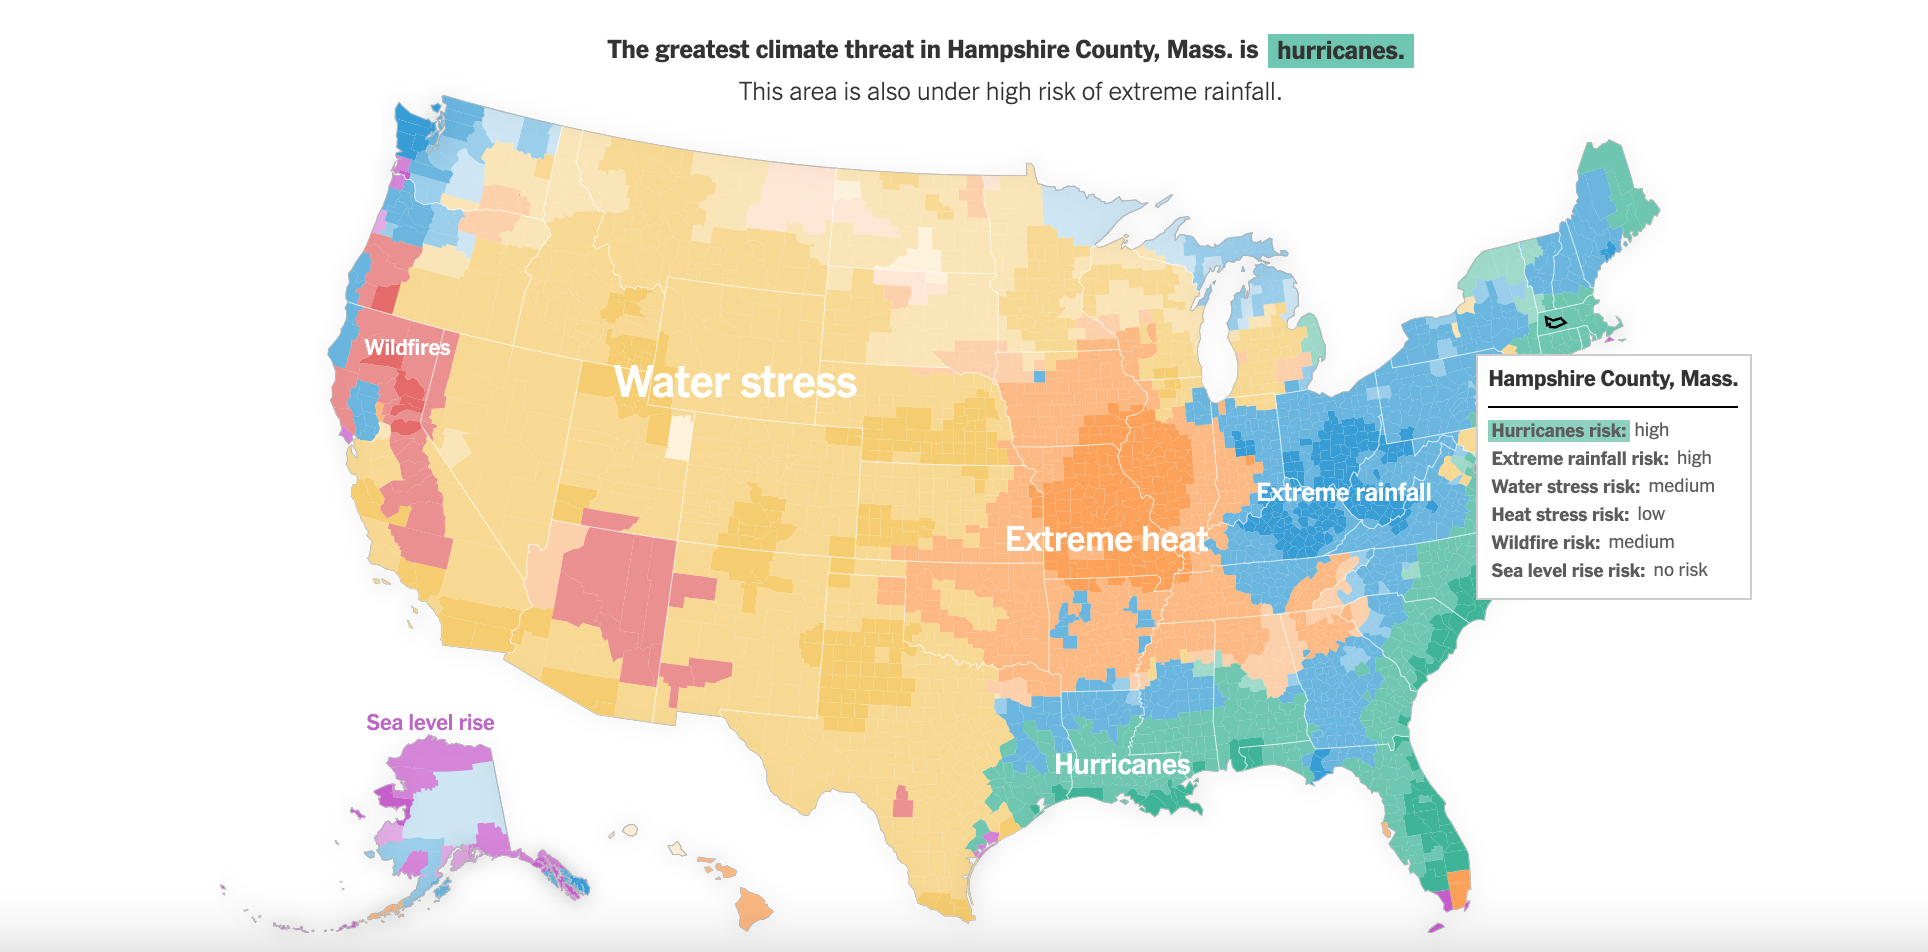
\includegraphics[width=0.8\linewidth]{images/NYT-climate-risk-map} 

}

\caption{New York Times climate risk map}\label{fig:unnamed-chunk-1}
\end{figure}

I am also a fan of the
\href{https://sharkresearch.rsmas.miami.edu/}{University of Miami Shark
Research Team's} maps that
\href{https://sharkresearch.rsmas.miami.edu/education/virtual-learning/tracking-sharks/}{show
the movements of each of the sharks} that they have tagged. I enjoy
following the path of one shark in particular, a 339cm female
\href{https://sharkresearch.rsmas.miami.edu/education/virtual-learning/tracking-sharks/olivia-eve/}{Tiger
shark called ``Olivia Eve''}, that is named after my friend Olivia.

\begin{figure}

{\centering 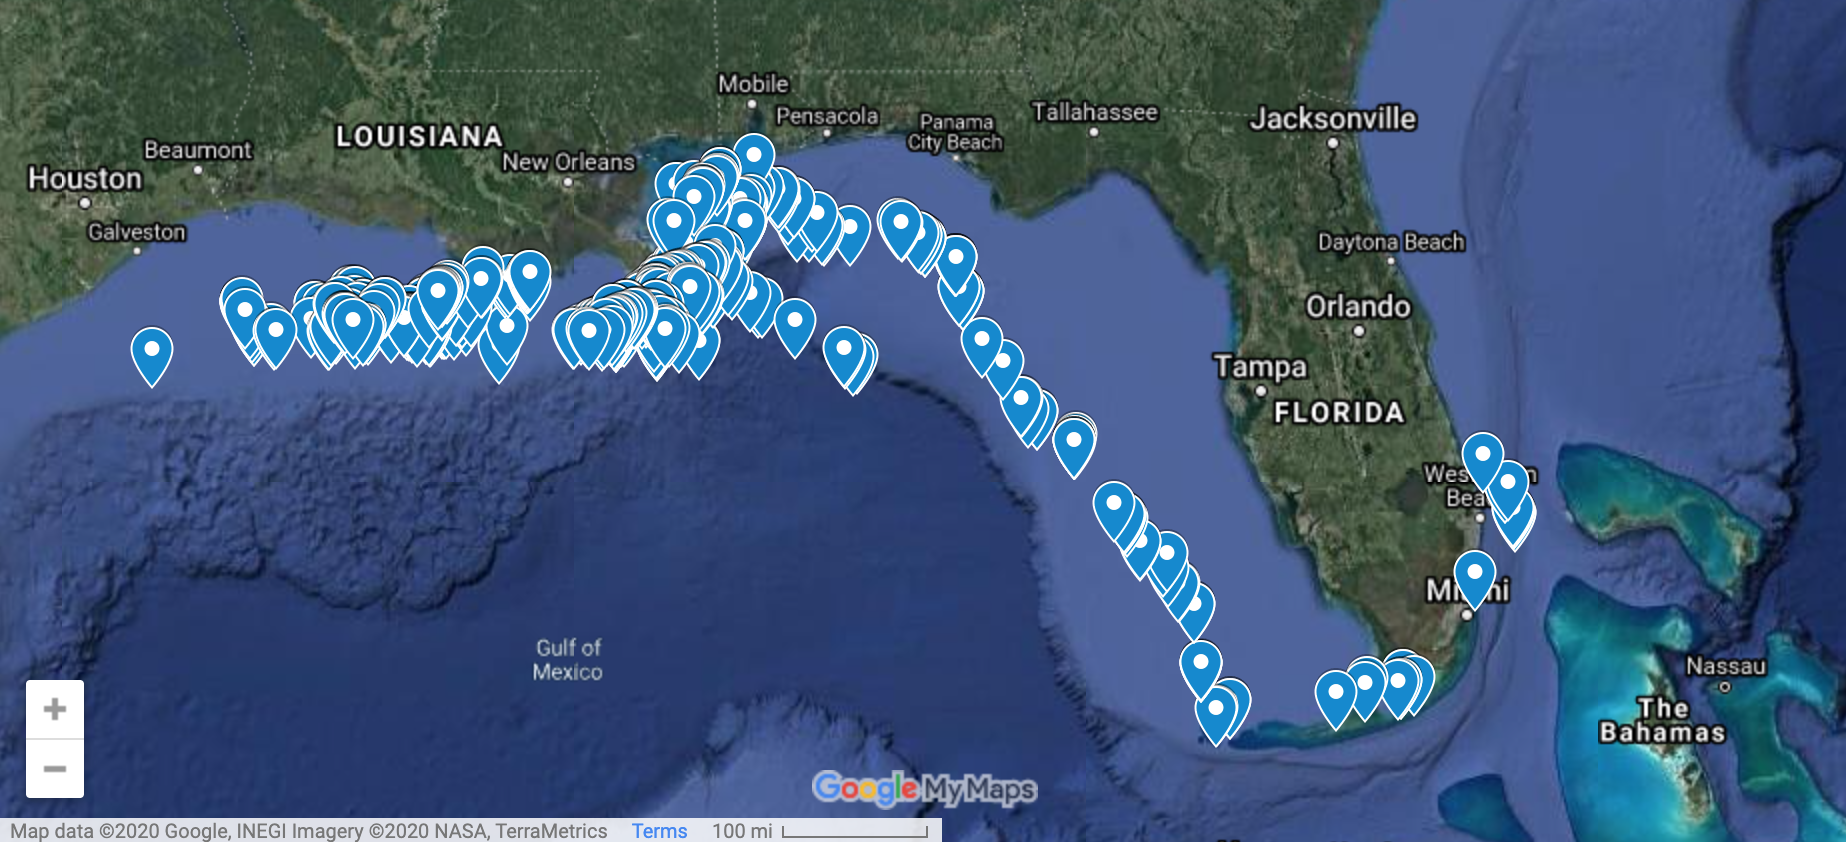
\includegraphics[width=0.8\linewidth]{images/olivia-eve-shark-map} 

}

\caption{Tracking the movements of Tiger shark Olivia Eve}\label{fig:unnamed-chunk-2}
\end{figure}

\hypertarget{why-work-with-geospatial-data-a-motivating-example}{%
\subsection{Why work with geospatial data? A motivating
example}\label{why-work-with-geospatial-data-a-motivating-example}}

Geospatial data is omnipresent in daily life and is ingrained into many
industries, but what about geospatial data makes it so appealing?
Depending upon who you ask, you may get a different answer, but the
following motivating example is intended to illustrate two particular
benefits of working with geospatial data. Visualizations made with
geospatial data allow us, at times, to process information in an easier
method than we could if we looked at the data in tabular format. As a
result, sometimes visual presentation can often lead to insights that
would otherwise be more difficult to conceptualize.

Consider the following example. Someone, perhaps a friend, asks you asks
you ``What is the climate of the United States?''. You know that there
is no one simple answer to this question - after all, it's no secret
that some places in the U.S. experience snow in December while other
places have warm tropical breezes at the same time.

Because there are so many places in the U.S. to consider, you realize
that you're going to need to be able to describe the climate of the U.S.
by looking at regions that are at least the size of states, if not
composed of multiple states so that you can provide a somewhat concise
response to your friend.

One approach you could take to answer your friend would be to primarily
consult tabular data. If you were to find a data set that listed every
U.S. census-designated location and its associated
\href{https://en.wikipedia.org/wiki/K\%C3\%B6ppen_climate_classification}{Köppen
climate type}, you could consider grouping the observations by state
\citep{wikipediaKoppenClimateClassification2020}. Then, you could
identify a way to declare an overall climate type for a given state, and
you could list the climate types of every state. While this approach may
theoretically be possible, it is ill-advised in practice. By taking this
approach, you would fail to identify that some states have multiple
climate types depending upon the region of the state. Furthermore, to
answer your friend, you'd be offering 50 climate types, which would
likely dizzy them and leave them feeling unsatisfied with your answer.

A preferred approach would be to make a map that shows the United States
with each census-designated place color-coded by Köppen climate type,
which you could then show to your friend. A benefit of the mapping
approach is that you would be able to point out that certain states have
multiple climate types. For example, the map below clearly indicates
that Arizona has multiple climate regions, including cold desert (BWk),
hot desert (BWh), hot-summer mediterranean (Csa), warm-summer
mediterrannean (Csb), cold semi-arid (Bsk), hot semi-arid (Bsh),
warm-summer mediterranean continental (Dsb), and hot-summer
mediterranean continental (Dsa). (See Appendix A for a legend indicating
what Köppen climate type each color of the map corresponds to).

\begin{figure}

{\centering 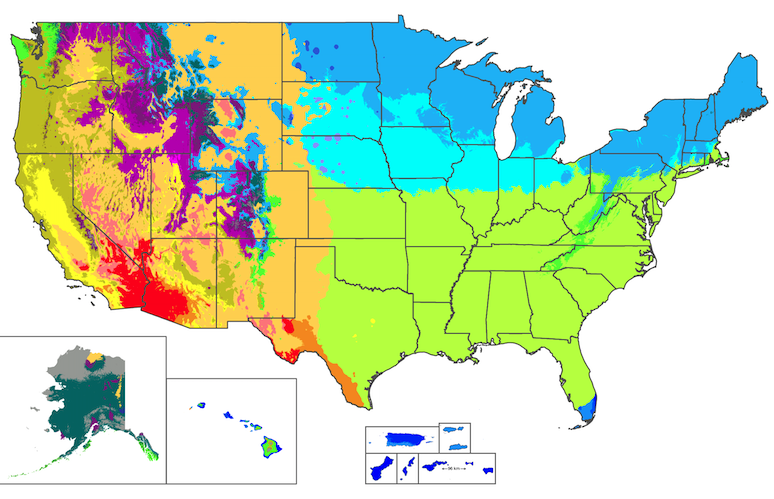
\includegraphics[width=0.75\linewidth]{images/US-climate-map} 

}

\caption{Köppen climate types of the U.S. (50 states, District of Columbia, and 5 inhabited U.S. territories}\label{fig:unnamed-chunk-3}
\end{figure}

Creating a map would also allow for you to show your friend that the
eastern half of the continguous United States has only a few climate
types, while the western half has numerous climate types. You could also
point out that there is a roughly horizontal line bisecting the eastern
half of the United States, with land above that line having either
warm-summer humid continental climate (Dfb) or hot-summer humid
continental climate (Dfa), and land below the line having humid
subtropical (Cfa), for the most part.

Your friend will likely be much happier that you chose to take advantage
of the fact that geospatial data lends itself to mapping instead of
limiting yourself to exploring geospatial data in a tabular format. As
this example illustrates, mapping geospatial data allows for individuals
to construct visual summaries and to have insights about patterns in the
data that they may not otherwise identify.

\hypertarget{shiny-app-trails-near-amherst-college}{%
\section{Shiny app: Trails Near Amherst
College}\label{shiny-app-trails-near-amherst-college}}

Given the ubiquity of geospatial data in life and the advantages that
geospatial data can provide when trying to extract meaning from data, I
was interested in spending my time for my final project starting to
learn about how to work with geospatial data.

I created a Shiny app, which can be
\href{https://nfrontero20.shinyapps.io/leaflet/}{accessed here}, that
displays what I have learned throughout this process. I will be
discussing the functionality of the app, as well as the geospatial
principles that I had to understand in order to make the app. To aid in
this explanation, I will be references images of the working
application.

\hypertarget{app-tabs-and-functionality}{%
\subsection{App tabs and
functionality}\label{app-tabs-and-functionality}}

The application has two main tabs, ``Map'' and ``Trail lengths,'' as
well as a third tab with background information on the project.

The map allows for users to select between three base layers, which are
tiles obtained through providers that Leaflet supports the use of
\citep{rstudioLeaflet}. Users can also choose to view additional layers,
which are the Amherst College trails and also railways throughout the
world. The Amherst College trails are displayed with permanent labels so
that a user can easily identify which trail is which. Finally, users can
zoom in and out of the app.

The second tab includes a table of the lengths of each of the Amherst
College trails, listed in both miles and kilometers. Users can search
for a trail name in a search bar.

As stated in the ``About'' tab of the app, my hope is, if this app was
shared with members of the Amherst community, that they would find it of
use by perhaps learning about the presence of trails they didn't know
existed, and by having a way to quickly identify the length of the
trails.

\begin{figure}

{\centering 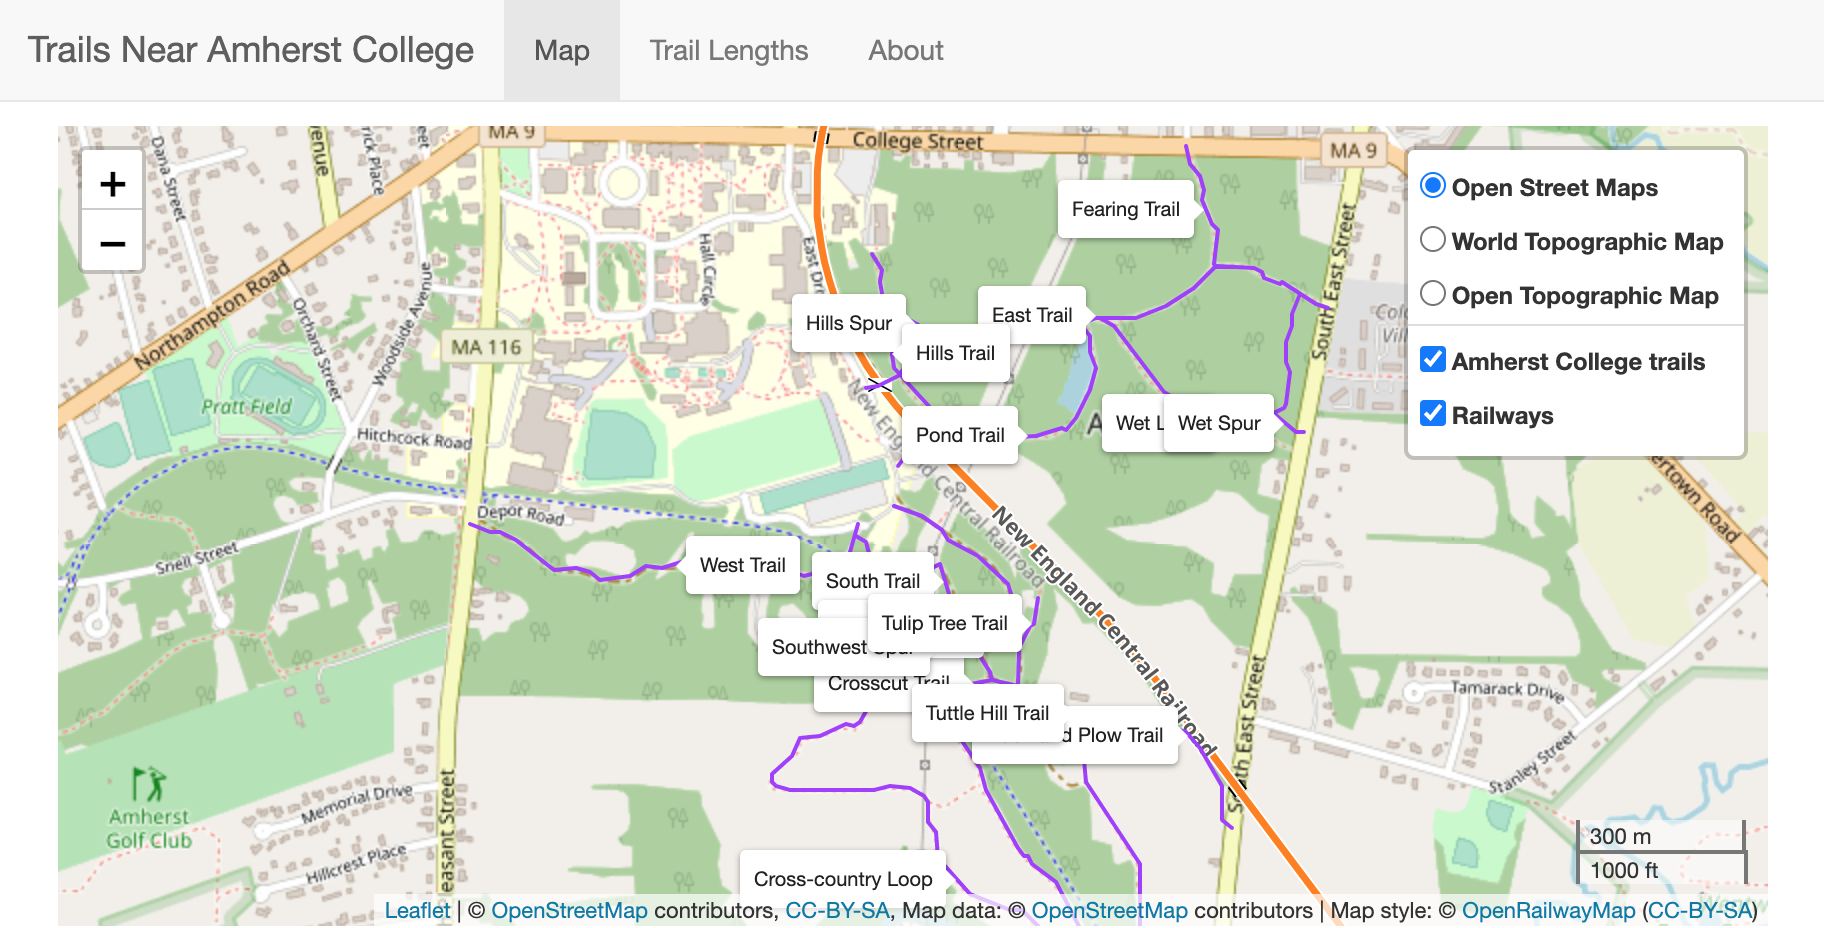
\includegraphics[width=0.9\linewidth]{images/screenshot-app-map} 

}

\caption{Map tab from the Shiny app}\label{fig:unnamed-chunk-4}
\end{figure}

\begin{figure}

{\centering 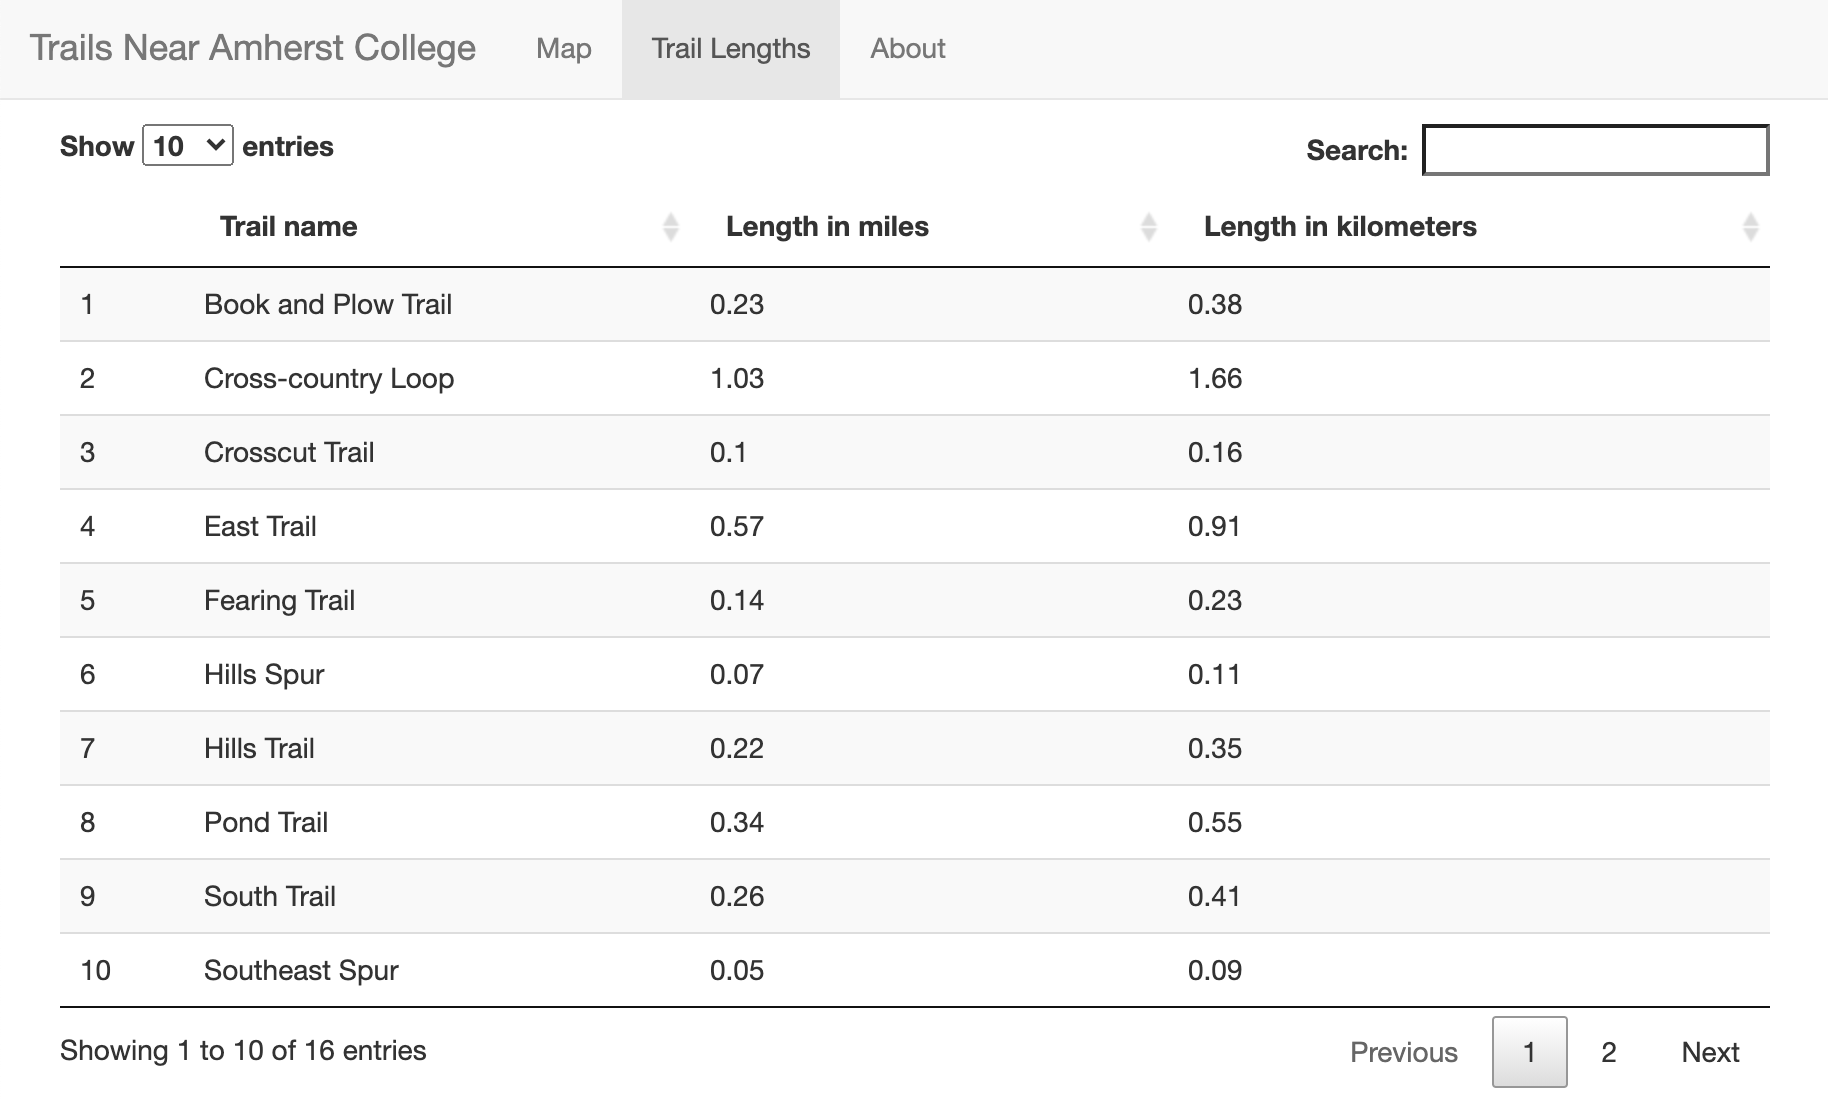
\includegraphics[width=0.9\linewidth]{images/screenshot-app-trail-lengths} 

}

\caption{Trail lengths tab from the Shiny app}\label{fig:unnamed-chunk-5}
\end{figure}

\hypertarget{behind-the-scenes}{%
\subsection{Behind the scenes}\label{behind-the-scenes}}

This app was created using methods of working with geospatial data in R.
I will provide information on the various geospatial topics that I
became acquainted with in order to make this app.

Geospatial data can be stored as either vectors or rasters, but in this
project I worked only with vector data. Vector data is geospatial data
that is stored as points, lines, and polygons
\citep{lovelaceGeocomputation2020}. The
\href{https://github.com/Amherst-STAT495F20/STAT495F20-project-Frontero/tree/main/data}{data
files} that I used contained vector data in
\href{https://en.wikipedia.org/wiki/Shapefile}{shapefiles} format. In
order to access a layer of data (data that could be added to a map),
four files with the same name but with different extensions are
required. The filetypes needed to work with shapefile data are .dbf,
.shp, .shx, and .prj.

I worked with three different data sets in this project.

\begin{itemize}
\item
  \textbf{Amherst College trails:} Obtained through
  \href{https://www.amherst.edu/offices/it}{Amherst College IT
  Department}.
\item
  \textbf{Bicycle trails:} Obtained through
  \href{https://docs.digital.mass.gov/massgis}{MassGIS (Massachusetts
  Bureau of Geographic Information)}. The specific layer I utilized is
  the
  \href{https://docs.digital.mass.gov/dataset/massgis-data-bicycle-trails}{Bicycle
  Trails} layer.
\item
  \textbf{Elevation contours:} Obtained through the
  \href{https://www.amherstma.gov/400/Amherst-Maps-Property-Info}{Amherst,
  MA town government website web-page dedicated to GIS data and maps of
  the town}. The data was downloaded using the Amherst, MA town
  government \href{http://gis.amherstma.gov/apps/topoextract.htm}{app to
  extract topographic data} by selecting the ``Elevation Contours''
  check box and downloading shapefiles.
\end{itemize}

In
\href{https://github.com/Amherst-STAT495F20/STAT495F20-project-Frontero/blob/main/create-objects.Rmd}{create-objects.rmd},
these data sets are read into R. The summary that prints when these
layers are read in tells us the geometry of the layers. As was just
mentioned, vector data is stored in points, lines, and polygons, and
there are combinations of these that produce different vector geometries
\citep{lovelaceGeocomputation2020}. Reading in these layers revealed
that the elevation contours layer has a geometry of type
\texttt{3D\ Line\ String}, and that the Amherst College trails and the
bike trails layers are of geometry type \texttt{Line\ String}.

I utilized the \texttt{sf::st\_read()} function to read in the layers.
\texttt{sf} offers quite a lot of versatility for manipulating layers,
but it ended up being that I only needed to use \texttt{sf::st\_read()}
when working with the layers. I would have used \texttt{sf::st\_crs()}
should it have proved necessary for me to reproject any of the layers.

This brings up another key geospatial data concept: projections.
Geospatial data is used to represent the three dimensional Earth in a
two dimensional space, such a computer screen or a book
\citep{hortonModernDataScience}. However, there is no simple way to
process of representing the three dimensional Earth in two dimensional
space. Consequently, there are many types of projections that differ in
various ways.

After the data was processed and all objects needed for the app were
saved to
\href{https://github.com/Amherst-STAT495F20/STAT495F20-project-Frontero/blob/main/shiny/app-objects.rda}{app-objects.rda},
the data was accessed via
\href{https://github.com/Amherst-STAT495F20/STAT495F20-project-Frontero/blob/main/shiny/Global.R}{Global.R}.
Placing the objects in Global.R allowed for
\href{https://github.com/Amherst-STAT495F20/STAT495F20-project-Frontero/blob/main/shiny/ui.R}{ui.R}
and
\href{https://github.com/Amherst-STAT495F20/STAT495F20-project-Frontero/blob/main/shiny/server.R}{server.R}
to have access to the objects because Global.R is a special file that
allows for the server and ui files to access any data that is in
Global.R without explicitly reading any data into the ui and server
files \citep{raessAwesomenessThatGlobal2018}.

\newpage

\hypertarget{conclusion}{%
\section{Conclusion}\label{conclusion}}

In this report I provided motivation for working with geospatial data,
commenting on the ubiquity of geospatial data in daily life. I offered a
motivating example of how geospatial data helps people construct visual
summaries and reach new insights about data that they likely wouldn't
have arrived at by just consulting tabular data. I then described my
study of geospatial data by showcasing the Shiny application that I made
and its functionality. I also provided ``behind the scenes'' information
on the coding that was necessary to create the app, and specifically the
geospatial concepts that were utilized.

As I reflect upon this project, I feel that the creation of the app and
this report has achieved a few key aims. First, this project allowed me
to showcase my statistics and data science acumen to date. But, arguably
more importantly, this project allowed me to learn about geospatial
data, an unfamiliar topic in the world of statistics and computing.
Finally, the creation of the app will hopefully serve as a resource to
individuals who want to engage in outdoor recreation near Amherst
College.

In terms of future directions, additional functionalities could be added
to the app. For example, creating elevation charts of the trails may be
a worthwhile pursuit. In fact, there is elevation contour data stored in
the Rdata file that is not currently incorporated into the app in any
way.

While this project represents a capstone product representative of my
statistics and data science acumen to date, I hope that years from now
when I look back upon this moment, I will see that I have grown even
more as a statistician from this date onward.

\newpage

\hypertarget{appendix}{%
\section{Appendix}\label{appendix}}

\begin{figure}

{\centering 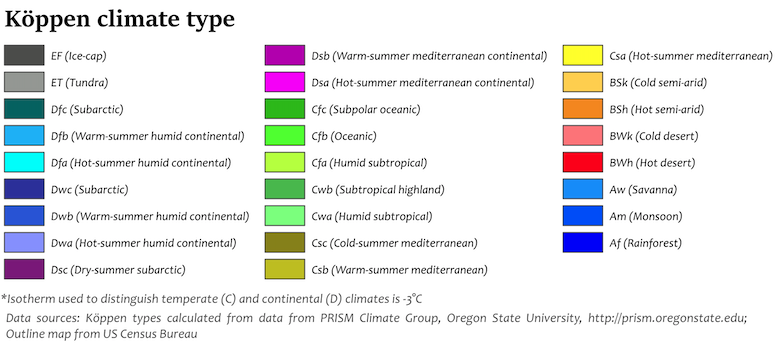
\includegraphics[width=0.9\linewidth]{images/koppen-climate-type-legend} 

}

\caption{Legend for figure 3 indicating Köppen climate types}\label{fig:unnamed-chunk-6}
\end{figure}

\bibliographystyle{agsm}
\bibliography{bibliography.bib}

\end{document}
